\documentclass[tikz,border=12pt]{standalone}
\usepackage{tikz}
\usetikzlibrary{positioning, arrows.meta, calc}

\definecolor{sig}{RGB}{60, 165, 110}
\definecolor{adapter}{RGB}{55, 175, 165}
\definecolor{msg}{RGB}{178, 102, 178}
\definecolor{model}{RGB}{120, 130, 160}
\definecolor{compl}{RGB}{200, 110, 110}
\definecolor{out}{RGB}{60, 165, 110}

\begin{document}
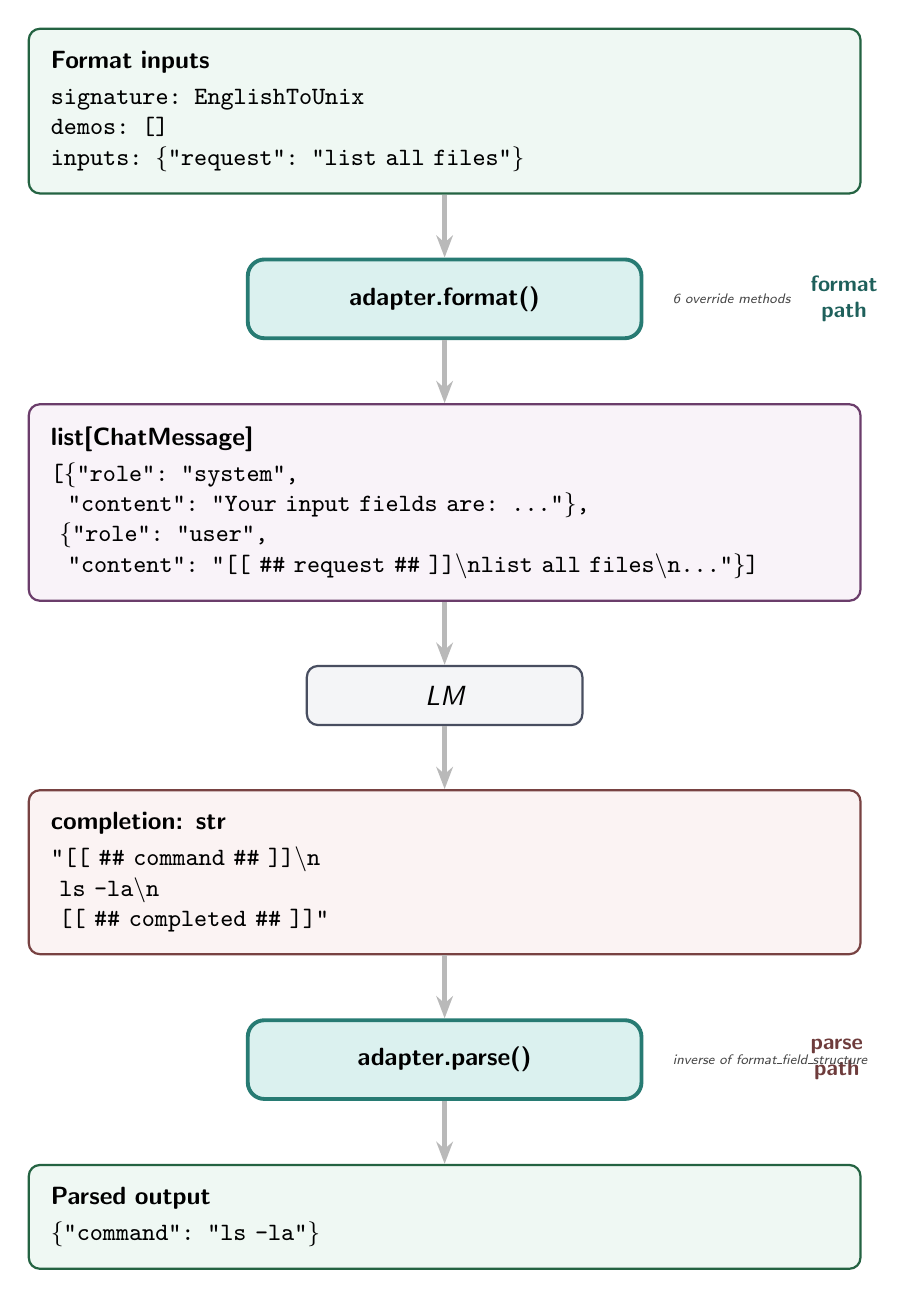
\begin{tikzpicture}[
    >=Stealth,
    font=\sffamily,
    iobox/.style={
        rectangle, rounded corners=4pt,
        draw=#1!60!black, fill=#1!8,
        line width=0.8pt, align=left,
        text width=10.0cm, inner sep=8pt,
        font=\sffamily\small,
    },
    adapt/.style={
        rectangle, rounded corners=6pt,
        draw=adapter!70!black, fill=adapter!18,
        line width=1.4pt, font=\sffamily\bfseries\small, align=center,
        minimum width=5cm, minimum height=1.0cm,
    },
    lmbox/.style={
        rectangle, rounded corners=4pt,
        draw=model!60!black, fill=model!8,
        line width=0.8pt, font=\sffamily\itshape, align=center,
        minimum width=3.5cm, minimum height=0.75cm,
    },
    arrow/.style={-{Stealth[length=8pt]}, line width=1.6pt, draw=gray!55},
    pathlabel/.style={
        font=\sffamily\footnotesize\bfseries,
        text=#1!55!black,
        align=center,
    },
    typecaption/.style={
        font=\sffamily\tiny\itshape, text=gray!55!black,
        anchor=west,
    },
    node distance=0.8cm and 0.4cm,
]

% =================================================
% TOP: Format path
% =================================================

\node[iobox=sig] (inpbox) {%
    \textbf{Format inputs}\\[2pt]
    \texttt{signature: EnglishToUnix}\\
    \texttt{demos: []}\\
    \texttt{inputs: \{"request": "list all files"\}}%
};

\node[adapt, below=of inpbox] (fmtcall) {adapter.format()};

\node[iobox=msg, below=of fmtcall] (msgbox) {%
    \textbf{list[ChatMessage]}\\[2pt]
    \texttt{[\{"role": "system",}\\
    \texttt{~~"content": "Your input fields are: ..."\},}\\
    \texttt{~\{"role": "user",}\\
    \texttt{~~"content": "[[ \#\# request \#\# ]]\textbackslash nlist all files\textbackslash n..."\}]}%
};

\node[lmbox, below=of msgbox] (lm) {LM};

% =================================================
% BOTTOM: Parse path
% =================================================

\node[iobox=compl, below=of lm] (complbox) {%
    \textbf{completion: str}\\[2pt]
    \texttt{"[[ \#\# command \#\# ]]\textbackslash n}\\
    \texttt{~ls -la\textbackslash n}\\
    \texttt{~[[ \#\# completed \#\# ]]"}%
};

\node[adapt, below=of complbox] (prscall) {adapter.parse()};

\node[iobox=out, below=of prscall] (outbox) {%
    \textbf{Parsed output}\\[2pt]
    \texttt{\{"command": "ls -la"\}}%
};

% =================================================
% Flow arrows
% =================================================
\draw[arrow] (inpbox)   -- (fmtcall);
\draw[arrow] (fmtcall)  -- (msgbox);
\draw[arrow] (msgbox)   -- (lm);
\draw[arrow] (lm)       -- (complbox);
\draw[arrow] (complbox) -- (prscall);
\draw[arrow] (prscall)  -- (outbox);

% =================================================
% Path labels on right side
% =================================================
\node[pathlabel=adapter, right=2.0cm of fmtcall] {format\\path};
\node[pathlabel=compl,   right=2.0cm of prscall] {parse\\path};

% =================================================
% Side annotations on adapter calls
% =================================================
\node[typecaption, right=0.25cm of fmtcall] {6 override methods};
\node[typecaption, right=0.25cm of prscall] {inverse of format\_field\_structure};

\end{tikzpicture}
\end{document}
